% ============================================================
%  MOEA/D Technical Report
%  Authors: Md. Rashidul Islam, Fathum Mobin, Md. Riyadun Nabi
% ============================================================
\documentclass[12pt,a4paper]{article}

% --- Packages ---
\usepackage[margin=1in, headheight=14.5pt]{geometry}
\usepackage{amsmath,amssymb,amsthm}
\usepackage{graphicx}
\usepackage{float}
\usepackage{booktabs}
\usepackage{array}
\usepackage{longtable}
\usepackage{multirow}
\usepackage{xcolor}
\usepackage{hyperref}
\usepackage{tikz}
\usetikzlibrary{shapes.geometric, arrows.meta, positioning, calc, fit, backgrounds}
\usepackage{pgfplots}
\pgfplotsset{compat=1.18}
\usepackage{caption}
\usepackage{subcaption}
\usepackage{enumitem}
\usepackage{setspace}
\usepackage{fancyhdr}
\usepackage{titlesec}
\usepackage{tocloft}
\usepackage{algorithm}
\usepackage{algpseudocode}
\usepackage{mdframed}
\usepackage{listings}
\usepackage{lipsum}
\usepackage{parskip}

% --- Colors ---
\definecolor{primaryblue}{RGB}{31,73,125}
\definecolor{accentblue}{RGB}{70,130,180}
\definecolor{lightgray}{RGB}{245,245,245}
\definecolor{darkgray}{RGB}{80,80,80}
\definecolor{paretored}{RGB}{192,0,0}

% --- Hyperref setup ---
\hypersetup{
    colorlinks=true,
    linkcolor=primaryblue,
    citecolor=primaryblue,
    urlcolor=accentblue,
    pdftitle={MOEA/D: Multi-Objective Evolutionary Algorithm based on Decomposition},
    pdfauthor={Md. Rashidul Islam, Fathum Mobin, Md. Riyadun Nabi}
}

% --- Header/Footer ---
\pagestyle{fancy}
\fancyhf{}
\fancyhead[L]{\small\textcolor{darkgray}{MOEA/D: Multi-Objective Evolutionary Algorithm based on Decomposition}}
\fancyhead[R]{\small\textcolor{darkgray}{\thepage}}
\fancyfoot[C]{\small\textcolor{darkgray}{Dept. of CSE --- Technical Report --- 2026}}
\renewcommand{\headrulewidth}{0.4pt}
\renewcommand{\footrulewidth}{0.4pt}

% --- Section formatting ---
\titleformat{\section}{\large\bfseries\color{primaryblue}}{{\thesection}}{1em}{}[\titlerule]
\titleformat{\subsection}{\normalsize\bfseries\color{accentblue}}{\thesubsection}{1em}{}
\titleformat{\subsubsection}{\normalsize\bfseries\color{darkgray}}{\thesubsubsection}{1em}{}

% --- TikZ styles ---
\tikzset{
    block/.style={rectangle, draw=primaryblue, fill=lightgray,
                  rounded corners, text centered, align=center, minimum height=1cm,
                  minimum width=2.8cm, font=\small},
    arrow/.style={-Stealth, thick, color=primaryblue},
    decision/.style={diamond, draw=paretored, fill=red!10,
                     text centered, align=center, minimum height=1cm,
                     minimum width=2cm, font=\small, aspect=2.5},
    startend/.style={ellipse, draw=primaryblue, fill=primaryblue!15,
                     text centered, align=center, minimum height=0.8cm,
                     minimum width=2cm, font=\small\bfseries}
}

% --- Theorem-like environments ---
\newmdtheoremenv[
  backgroundcolor=lightgray,
  linecolor=primaryblue,
  linewidth=1.5pt,
  topline=false, rightline=false, bottomline=false
]{definition}{Definition}

\newmdtheoremenv[
  backgroundcolor=red!5,
  linecolor=paretored,
  linewidth=1.5pt,
  topline=false, rightline=false, bottomline=false
]{theorem}{Theorem}

% =============================================================
\begin{document}

% ---- Title Page ----
\begin{titlepage}
    \centering
    \vspace*{1cm}
    {\Huge\bfseries\color{primaryblue}
     Multi-Objective Evolutionary\\[0.3em]
     Algorithm based on Decomposition\\[0.3em]
     \textbf{(MOEA/D)}\par}
    \vspace{0.5cm}
    \rule{\linewidth}{1.5pt}
    \vspace{0.3cm}
    {\large\itshape A Technical Report Submitted in Partial Fulfillment\\
     of the Course Requirements\par}
    \vspace{1.5cm}

    {\large\bfseries Submitted by\par}
    \vspace{0.5cm}
    \begin{tabular}{ll}
        \textbf{Md. Rashidul Islam} & \textbf{ID: 2205072} \\[4pt]
        \textbf{Fathum Mobin}       & \textbf{ID: 2205073} \\[4pt]
        \textbf{Md. Riyadun Nabi}   & \textbf{ID: 2205076} \\
    \end{tabular}

    \vspace{1.5cm}
    {\large\bfseries Submitted to\par}
    \vspace{0.3cm}
    {\large Course Instructor\\
     Department of Computer Science and Engineering\par}

    \vspace{1.5cm}
    % \includegraphics[width=0.25\textwidth]{university_logo}
    % PLACEHOLDER: Replace "university_logo" with your university logo file (e.g., logo.png)
    % \includegraphics[width=0.25\textwidth]{your_logo.png}

    \vspace{1cm}
    {\large April 2026\par}
    \vspace{0.5cm}
    \rule{\linewidth}{1pt}
\end{titlepage}

% ---- Abstract ----
\newpage
\begin{abstract}
\noindent
Multi-objective optimization problems (MOPs) arise in virtually every engineering and scientific domain --- from training machine learning models to designing energy-efficient vehicles. These problems require the simultaneous optimization of two or more conflicting objectives, where improving one goal typically degrades another. Classical single-objective methods are fundamentally ill-suited to discover the full spectrum of trade-off solutions known as the \emph{Pareto front}.

This report presents a comprehensive study of \textbf{MOEA/D} (Multi-Objective Evolutionary Algorithm based on Decomposition), an elegant and computationally efficient framework proposed by Zhang and Li (2007). The core philosophy of MOEA/D is to decompose the original multi-objective problem into $N$ scalar subproblems, each defined by a distinct weight vector $\boldsymbol{\lambda}^i$, and to solve these subproblems simultaneously by exploiting neighborhood relationships. Each subproblem is solved using a scalarization function --- either the Weighted Sum (WS) or the Tchebycheff (TCH) approach --- which converts the multi-dimensional objective vector into a single comparable scalar score.

We explain the theoretical foundations of Pareto optimality, dominance, and Pareto fronts; detail the two main scalarization strategies; describe the MOEA/D algorithm step by step with pseudocode and flowcharts; and discuss the key design choices such as neighborhood size, weight vector generation, and the ideal reference point. The report is enriched with intuitive real-world analogies, illustrative examples, and comparative tables to make the material accessible while remaining rigorous.
\end{abstract}

\vspace{1cm}
\noindent\textbf{Keywords:} Multi-objective optimization, Pareto front, evolutionary algorithm, decomposition, scalarization, weight vectors, Tchebycheff, NSGA-II, neighborhood cooperation.

% ---- Table of Contents ----
\newpage
\tableofcontents
\listoffigures
\listoftables
\newpage

% =============================================================
\section{Introduction}
% =============================================================

Optimization is at the heart of engineering and science. We seek the ``best'' solution among all feasible candidates. For decades, this search was treated as a single-number problem: minimize cost, maximize accuracy, or find the shortest path. However, almost every real decision involves multiple, competing objectives at once.

Consider a few everyday examples:
\begin{itemize}[leftmargin=1.5cm]
    \item \textbf{Buying a car:} You want maximum speed \emph{and} minimum fuel consumption. A sports car gives you speed but drinks fuel; an economy car saves fuel but is slow.
    \item \textbf{Machine learning:} You want a model that is both \emph{accurate} and \emph{fast to run}. High-accuracy deep networks are computationally expensive; lightweight models sacrifice accuracy.
    \item \textbf{Finance:} You want \emph{high return} with \emph{low risk}. Higher-return investments tend to be riskier.
\end{itemize}

In all these cases, there is no single ``perfect'' answer. There is a \emph{set} of excellent answers, each representing a different trade-off. Finding this entire set --- called the \textbf{Pareto front} --- is the fundamental goal of multi-objective optimization.

Classical methods such as gradient descent, linear programming, or even single-objective evolutionary algorithms can find at most \emph{one} solution per run. To get different trade-off points, a practitioner must manually re-tune weights and re-run from scratch --- an expensive and impractical process.

\textbf{MOEA/D}, proposed by Qingfu Zhang and Hui Li in 2007, solves this inefficiency with a brilliantly simple idea: \emph{decompose} the multi-objective problem into many scalar subproblems, each optimized from a different ``preference direction'', and let these subproblems \emph{cooperate} by sharing useful information with their neighbors. In a single run, MOEA/D approximates the entire Pareto front.

\subsection{Motivation}

Table~\ref{tab:classical_vs_moead} contrasts classical single-objective methods against MOEA/D to highlight the need for the algorithm.

\begin{table}[H]
\centering
\caption{Classical Optimization vs.\ MOEA/D}
\label{tab:classical_vs_moead}
\renewcommand{\arraystretch}{1.4}
\begin{tabular}{>{\bfseries}p{4cm} p{5cm} p{5cm}}
\toprule
\textbf{Aspect} & \textbf{Classical / Single-Objective} & \textbf{MOEA/D} \\
\midrule
Output per run & One solution & Full approximation of Pareto front \\
Trade-off exploration & Must rerun with different weights & All trade-offs explored simultaneously \\
Handling conflicts & Collapses objectives to one & Preserves objective structure \\
Diversity of solutions & Low (single point) & High (population spread across front) \\
Scalability & Good for 1--2 objectives & Good for 2--4 objectives \\
Mechanism & Gradient / exact methods & Evolutionary + decomposition \\
\bottomrule
\end{tabular}
\end{table}

\subsection{Scope of This Report}

This report is organized as follows. Section~\ref{sec:mop} introduces the formal definition of a multi-objective optimization problem. Section~\ref{sec:pareto} explains the concept of dominance and the Pareto front. Section~\ref{sec:ea} reviews evolutionary algorithms and why they are natural candidates for MOPs. Section~\ref{sec:decomp} explains the decomposition idea via intuitive analogies. Section~\ref{sec:scalarization} covers the two major scalarization approaches used in MOEA/D. Section~\ref{sec:algorithm} gives the full algorithm with pseudocode and a flowchart. Section~\ref{sec:design} discusses key design parameters. Section~\ref{sec:comparison} compares MOEA/D with related algorithms. Section~\ref{sec:applications} lists real-world application domains. Section~\ref{sec:conclusion} concludes.

% =============================================================
\section{Multi-Objective Optimization Problems}
\label{sec:mop}
% =============================================================

\subsection{Formal Definition}

A multi-objective optimization problem (MOP) in minimization form is defined as:

\begin{equation}
    \min_{\mathbf{x} \in \Omega} \; \mathbf{F}(\mathbf{x})
    = \bigl(f_1(\mathbf{x}),\; f_2(\mathbf{x}),\; \ldots,\; f_m(\mathbf{x})\bigr)
    \label{eq:mop}
\end{equation}

where:
\begin{itemize}[leftmargin=1.5cm]
    \item $\mathbf{x} = (x_1, x_2, \ldots, x_n) \in \Omega \subseteq \mathbb{R}^n$ is the \textbf{decision variable vector} in the \emph{decision space} $\Omega$,
    \item $f_k : \Omega \to \mathbb{R}$ is the $k$-th objective function for $k = 1, \ldots, m$,
    \item $\mathbf{F} : \Omega \to \mathbb{R}^m$ maps a decision vector to an \textbf{objective vector} in the \emph{objective space}.
\end{itemize}

The problem may additionally include constraints:
\begin{equation}
    g_j(\mathbf{x}) \leq 0, \quad j = 1, \ldots, p, \qquad
    h_k(\mathbf{x}) = 0, \quad k = 1, \ldots, q.
\end{equation}

\subsection{Why Objectives Conflict}

The challenge arises because the individual minima of $f_1, f_2, \ldots, f_m$ generally cannot be achieved simultaneously. Formally, let $\mathbf{x}_k^* = \arg\min_{\mathbf{x}} f_k(\mathbf{x})$. For most real problems, $\mathbf{x}_1^* \neq \mathbf{x}_2^* \neq \cdots \neq \mathbf{x}_m^*$. This means that improving $f_1$ (moving toward $\mathbf{x}_1^*$) tends to increase some $f_j$ for $j \neq 1$.

\subsection{Illustrative Example: Machine Learning Model Selection}

Suppose we train three models on the same dataset. Table~\ref{tab:ml_models} shows their performance profiles.

\begin{table}[H]
\centering
\caption{Three ML models with conflicting accuracy--speed trade-offs}
\label{tab:ml_models}
\renewcommand{\arraystretch}{1.3}
\begin{tabular}{cccc}
\toprule
\textbf{Model} & \textbf{Accuracy (\%)} & \textbf{Inference Speed} & \textbf{Memory (MB)} \\
\midrule
Model A & 98 & Slow   & 512 \\
Model B & 90 & Very Fast & 64  \\
Model C & 95 & Medium    & 128 \\
\bottomrule
\end{tabular}
\end{table}

Which model is ``best''? If accuracy is the only concern, choose A. If deployment on a mobile device matters, choose B. For a balanced requirement, choose C. There is no universal winner --- the answer depends on the application context. This is precisely the essence of a multi-objective problem.

% =============================================================
\section{Pareto Optimality}
\label{sec:pareto}
% =============================================================

\subsection{Dominance Relation}

\begin{definition}[Pareto Dominance]
A solution $\mathbf{x}^{(1)}$ is said to \textbf{dominate} $\mathbf{x}^{(2)}$ (written $\mathbf{x}^{(1)} \prec \mathbf{x}^{(2)}$) if and only if:
\begin{align}
    &f_k(\mathbf{x}^{(1)}) \leq f_k(\mathbf{x}^{(2)}) \quad \forall\, k \in \{1, \ldots, m\} \quad \text{(no worse in all objectives)}, \label{eq:dom1}\\
    &\exists\, j \in \{1, \ldots, m\} \text{ such that } f_j(\mathbf{x}^{(1)}) < f_j(\mathbf{x}^{(2)}) \quad \text{(strictly better in at least one)}.
    \label{eq:dom2}
\end{align}
\end{definition}

Informally: $\mathbf{x}^{(1)}$ dominates $\mathbf{x}^{(2)}$ when it is at least as good as $\mathbf{x}^{(2)}$ in every objective \emph{and} strictly better in at least one. A dominated solution can be safely discarded.

\subsection{Non-Domination and the Pareto Front}

\begin{definition}[Pareto Optimal Solution]
A solution $\mathbf{x}^* \in \Omega$ is \textbf{Pareto optimal} if there exists no other $\mathbf{x} \in \Omega$ such that $\mathbf{x} \prec \mathbf{x}^*$.
\end{definition}

\begin{definition}[Pareto Front]
The \textbf{Pareto front} (PF) is the image of all Pareto optimal solutions in the objective space:
\begin{equation}
    \text{PF} = \bigl\{ \mathbf{F}(\mathbf{x}^*) \mid \mathbf{x}^* \text{ is Pareto optimal} \bigr\}.
\end{equation}
\end{definition}

The Pareto front is the set of all non-dominated objective vectors. It represents the complete picture of achievable trade-offs.

\subsection{Car Selection Example: Dominance in Action}

Consider four candidate cars with the objective of \emph{maximizing speed} and \emph{minimizing fuel use} (both converted to minimization: we minimize $-\text{speed}$ and minimize fuel).

\begin{table}[H]
\centering
\caption{Four candidate cars and dominance analysis}
\label{tab:cars}
\renewcommand{\arraystretch}{1.3}
\begin{tabular}{ccccc}
\toprule
\textbf{Car} & \textbf{Speed (km/h)} & \textbf{Fuel (L/100 km)} & \textbf{Dominated by} & \textbf{Status} \\
\midrule
A & 300 & 10 & --- & Non-dominated \\
B & 220 & 6  & --- & Non-dominated \\
C & 150 & 4  & --- & Non-dominated \\
D & 200 & 9  & B   & \textbf{Dominated} \\
\bottomrule
\end{tabular}
\end{table}

Car D is dominated by Car B because B achieves higher speed (220 > 200) \emph{and} lower fuel consumption (6 < 9). Cars A, B, and C are mutually non-dominated and collectively form the Pareto front for this example.

\subsection{Visualization of the Pareto Front}

\begin{figure}[H]
\centering
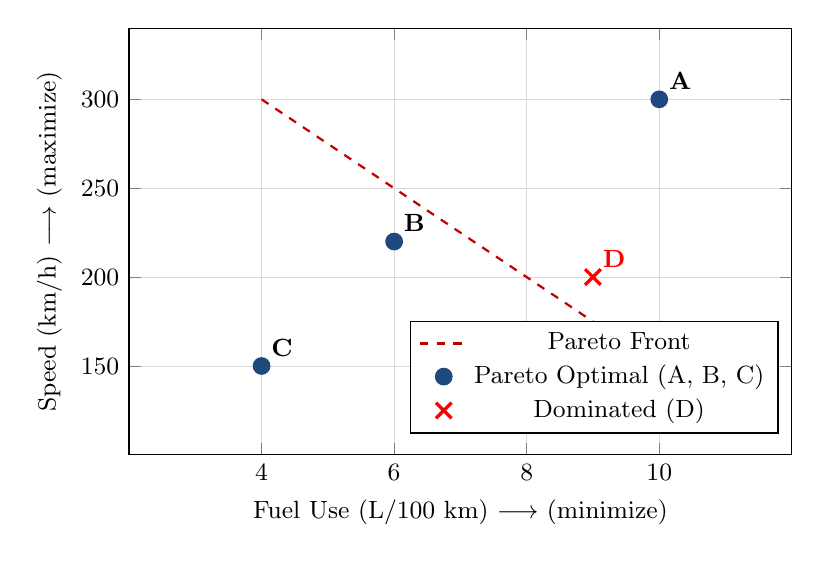
\begin{tikzpicture}
\begin{axis}[
    width=10cm, height=7cm,
    xlabel={Fuel Use (L/100 km) $\longrightarrow$ (minimize)},
    ylabel={Speed (km/h) $\longrightarrow$ (maximize)},
    xmin=2, xmax=12, ymin=100, ymax=340,
    xtick={4,6,8,10}, ytick={150,200,250,300},
    grid=both, grid style={line width=0.3pt, gray!30},
    tick label style={font=\small},
    label style={font=\small},
    legend style={font=\small, at={(0.98,0.05)}, anchor=south east}
]
% Pareto front curve
\addplot[thick, color=paretored, dashed, domain=4:10, samples=50]
    {150 + (300-150)*((10-x)/6)};
\addlegendentry{Pareto Front}

% Points
\addplot[only marks, mark=*, mark size=3pt, color=primaryblue]
    coordinates {(10,300)(6,220)(4,150)};
\addlegendentry{Pareto Optimal (A, B, C)}

\addplot[only marks, mark=x, mark size=4pt, very thick, color=red]
    coordinates {(9,200)};
\addlegendentry{Dominated (D)}

% Labels
\node[above right, font=\small\bfseries] at (axis cs:10,300) {A};
\node[above right, font=\small\bfseries] at (axis cs:6,220)  {B};
\node[above right, font=\small\bfseries] at (axis cs:4,150)  {C};
\node[above right, font=\small\bfseries, color=red] at (axis cs:9,200) {D};
\end{axis}
\end{tikzpicture}
\caption{Pareto front in objective space for the car selection example. Car D (red cross) is dominated; Cars A, B, C form the Pareto front (blue dots).}
\label{fig:pareto_car}
\end{figure}

% =============================================================
\section{Evolutionary Algorithms for Multi-Objective Problems}
\label{sec:ea}
% =============================================================

\subsection{Why Evolutionary Algorithms?}

Classical optimization methods (gradient descent, linear programming) find a single solution per run and require differentiable or linear objective functions. Evolutionary Algorithms (EAs) operate on a \emph{population} of candidate solutions simultaneously, which makes them naturally suited to approximate the Pareto front in one pass.

The three-step evolutionary cycle is:

\begin{enumerate}[leftmargin=1.5cm]
    \item \textbf{Selection:} Solutions with better fitness scores have a higher probability of being chosen as parents for the next generation.
    \item \textbf{Variation (Crossover + Mutation):} Parents are combined (crossover) and small random changes are introduced (mutation) to create offspring. Crossover mixes existing traits; mutation introduces new genetic material to prevent stagnation.
    \item \textbf{Replacement:} Offspring replace members of the current population according to a fitness-based criterion. The cycle repeats until a termination condition is met.
\end{enumerate}

\subsection{The Evolutionary Cycle Illustrated}

\begin{figure}[H]
\centering
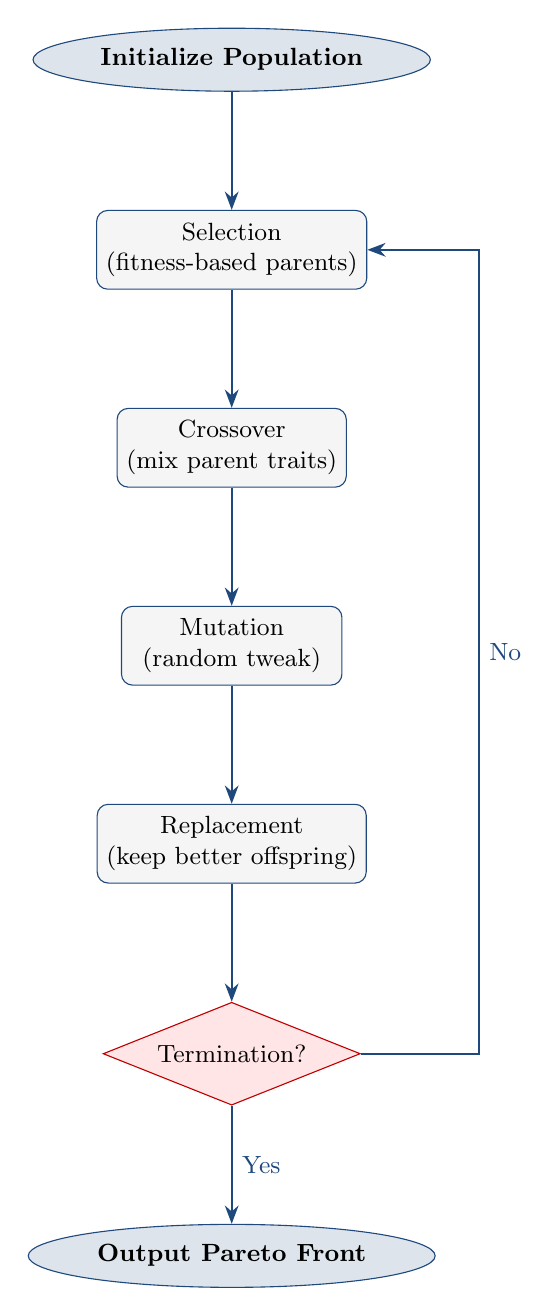
\begin{tikzpicture}[node distance=1.5cm]
    \node[startend] (init) {Initialize Population};
    \node[block, below=of init] (sel) {Selection\\(fitness-based parents)};
    \node[block, below=of sel] (cross) {Crossover\\(mix parent traits)};
    \node[block, below=of cross] (mut) {Mutation\\(random tweak)};
    \node[block, below=of mut] (rep) {Replacement\\(keep better offspring)};
    \node[decision, below=of rep] (stop) {Termination?};
    \node[startend, below=of stop] (out) {Output Pareto Front};

    \draw[arrow] (init) -- (sel);
    \draw[arrow] (sel) -- (cross);
    \draw[arrow] (cross) -- (mut);
    \draw[arrow] (mut) -- (rep);
    \draw[arrow] (rep) -- (stop);
    \draw[arrow] (stop) -- node[right]{\small Yes} (out);
    \draw[arrow] (stop.east) -- ++(1.5,0) |- node[right, near start]{\small No} (sel.east);
\end{tikzpicture}
\caption{The standard evolutionary cycle used in population-based algorithms.}
\label{fig:ea_cycle}
\end{figure}

\subsection{Crossover and Mutation in Detail}

\textbf{Crossover} takes two parent solutions and combines their components. If parents are represented as real-valued vectors $\mathbf{p}_1 = (p_1^1, \ldots, p_1^n)$ and $\mathbf{p}_2 = (p_2^1, \ldots, p_2^n)$, a typical Simulated Binary Crossover (SBX) produces children by interpolation:
\begin{equation}
    c_k^{(1)} = \tfrac{1}{2}\bigl[(1 + \beta_k)\,p_1^k + (1 - \beta_k)\,p_2^k\bigr],
    \quad
    c_k^{(2)} = \tfrac{1}{2}\bigl[(1 - \beta_k)\,p_1^k + (1 + \beta_k)\,p_2^k\bigr],
\end{equation}
where $\beta_k$ is a spread factor drawn from a distribution controlled by a distribution index $\eta_c$.

\textbf{Mutation} (e.g., polynomial mutation) perturbs a child component:
\begin{equation}
    c_k' = c_k + \delta_k \cdot (c_k^{(\max)} - c_k^{(\min)}),
\end{equation}
where $\delta_k$ is a small polynomial perturbation and $[c_k^{(\min)}, c_k^{(\max)}]$ is the feasible range.

\subsection{Why EAs Are Natural for MOPs}

\begin{table}[H]
\centering
\caption{EA characteristics that benefit multi-objective search}
\label{tab:ea_moea}
\renewcommand{\arraystretch}{1.3}
\begin{tabular}{p{4.5cm} p{9cm}}
\toprule
\textbf{EA Property} & \textbf{Why It Helps MOPs} \\
\midrule
Population-based & Multiple solutions explored per iteration --- naturally maps to the Pareto front. \\
Stochastic & Can escape local optima; explores a wider objective landscape. \\
Gradient-free & Works with non-differentiable, non-convex objective functions. \\
No single-solution bias & All population members are potential Pareto candidates. \\
One run, many solutions & Full Pareto approximation in a single optimization run. \\
\bottomrule
\end{tabular}
\end{table}

% =============================================================
\section{The Idea of Decomposition}
\label{sec:decomp}
% =============================================================

\subsection{From One Hard Problem to Many Easy Ones}

The core insight of MOEA/D is elegantly simple: instead of trying to simultaneously optimize all objectives in one complex search, we \textbf{decompose} the multi-objective problem into $N$ scalar subproblems, each encoding a specific preference direction over the objectives. Mathematically:

\begin{equation}
    \text{MOP} \;\xrightarrow{\text{decompose}}\; g^1(\mathbf{x}\mid\boldsymbol{\lambda}^1),\;
    g^2(\mathbf{x}\mid\boldsymbol{\lambda}^2),\; \ldots,\;
    g^N(\mathbf{x}\mid\boldsymbol{\lambda}^N)
\end{equation}

where each $g^i$ is a \emph{scalar} function parameterized by a weight vector $\boldsymbol{\lambda}^i \in \mathbb{R}^m$ with $\sum_{k=1}^m \lambda^i_k = 1$ and $\lambda^i_k \geq 0$.

\subsection{Analogy: University Scholarship Selection}

Imagine you are on a scholarship selection committee reviewing 2,000 applicants. Each applicant is described by four criteria: CGPA, Research output, Leadership, and Financial need. How do you rank them?

Trying to build a single global ranking fails because:
\begin{enumerate}[leftmargin=1.5cm]
    \item Different committee members have different priorities (some value CGPA; others value financial need).
    \item A single ranking tends to favor whoever excels at the most heavily weighted criterion --- leaving deserving candidates in other dimensions unrecognized.
    \item With 2,000 applicants and 4 criteria, the number of pairwise comparisons is approximately $\binom{2000}{2} \approx 2 \times 10^6$ --- computationally and conceptually unwieldy.
\end{enumerate}

The better approach is to define \emph{separate} sub-rankings, each emphasizing a different preference:
\begin{itemize}[leftmargin=1.5cm]
    \item $g_1$: CGPA-focused subproblem
    \item $g_2$: Research-focused subproblem
    \item $g_3$: Leadership-focused subproblem
    \item $g_4$: Need-focused subproblem
    \item $g_5$: Balanced subproblem
\end{itemize}

Each sub-ranking is simple to compute. Together, they cover the full diversity of deserving candidates --- exactly what a fair process requires. This is \textbf{decomposition}.

\subsection{Analogy: Phone Store — Weight Vectors in Action}

Consider choosing a smartphone on two criteria: price (minimize) and camera quality (maximize, converted to minimization as $-\text{camera}$). Four phones are on display (Table~\ref{tab:phones}).

\begin{table}[H]
\centering
\caption{Smartphone candidates and their Pareto status}
\label{tab:phones}
\renewcommand{\arraystretch}{1.3}
\begin{tabular}{ccccc}
\toprule
\textbf{Phone} & \textbf{Price (USD)} & \textbf{Camera (out of 5)} & \textbf{Dominated?} & \textbf{Best for} \\
\midrule
A & 200  & 2/5 & No  & Tight budget \\
B & 450  & 4/5 & No  & Balanced     \\
C & 1100 & 5/5 & No  & Best camera  \\
D & 500  & 2/5 & \textbf{Yes} (by B) & --- \\
\bottomrule
\end{tabular}
\end{table}

Phone D is dominated: Phone B beats it on \emph{both} objectives (lower price \emph{and} better camera). Phones A, B, C form the Pareto front. A weight vector $\boldsymbol{\lambda} = (\lambda_1, \lambda_2)$ encodes the preference between price and camera quality:

\begin{equation}
    \lambda_1 + \lambda_2 = 1, \quad \lambda_1, \lambda_2 \geq 0.
\end{equation}

\begin{itemize}[leftmargin=1.5cm]
    \item $\boldsymbol{\lambda} = (0.9, 0.1)$: 90\% weight on price $\Rightarrow$ finds Phone A.
    \item $\boldsymbol{\lambda} = (0.5, 0.5)$: balanced preference $\Rightarrow$ finds Phone B.
    \item $\boldsymbol{\lambda} = (0.1, 0.9)$: 90\% weight on camera $\Rightarrow$ finds Phone C.
\end{itemize}

Each weight vector is a \textbf{search direction} in objective space. Assigning many evenly spread weight vectors ensures that all regions of the Pareto front are covered.

\subsection{Geometric Interpretation of Weight Vectors}

Figure~\ref{fig:weight_vectors} illustrates how weight vectors $\boldsymbol{\lambda}^1, \ldots, \boldsymbol{\lambda}^5$ define search directions in the objective space, each pointing toward a different region of the Pareto front.

\begin{figure}[H]
\centering
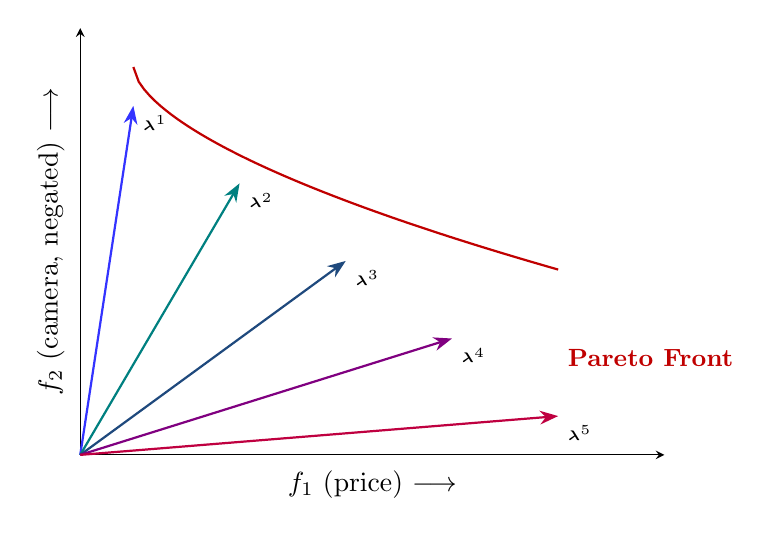
\begin{tikzpicture}
\begin{axis}[
    width=9cm, height=7cm,
    xlabel={$f_1$ (price) $\longrightarrow$},
    ylabel={$f_2$ (camera, negated) $\longrightarrow$},
    xmin=0, xmax=11, ymin=0, ymax=11,
    xtick=\empty, ytick=\empty,
    axis lines=left,
    clip=false
]
% Pareto front (convex curve)
\addplot[thick, color=paretored, domain=1:9, samples=80]
    {10 - (x-1)^(0.6)*1.5};
\node[right, color=paretored, font=\small\bfseries] at (axis cs:9,2.5) {Pareto Front};

% Weight vector directions from origin
\draw[-Stealth, thick, color=blue!80] (axis cs:0,0) -- (axis cs:1,9);
\draw[-Stealth, thick, color=teal] (axis cs:0,0) -- (axis cs:3,7);
\draw[-Stealth, thick, color=primaryblue] (axis cs:0,0) -- (axis cs:5,5);
\draw[-Stealth, thick, color=violet] (axis cs:0,0) -- (axis cs:7,3);
\draw[-Stealth, thick, color=purple] (axis cs:0,0) -- (axis cs:9,1);
\node[font=\tiny, below right] at (axis cs:1,9)   {$\boldsymbol{\lambda}^1$};
\node[font=\tiny, below right] at (axis cs:3,7)   {$\boldsymbol{\lambda}^2$};
\node[font=\tiny, below right] at (axis cs:5,5)   {$\boldsymbol{\lambda}^3$};
\node[font=\tiny, below right] at (axis cs:7,3)   {$\boldsymbol{\lambda}^4$};
\node[font=\tiny, below right] at (axis cs:9,1)   {$\boldsymbol{\lambda}^5$};
\end{axis}
\end{tikzpicture}
\caption{Weight vectors $\boldsymbol{\lambda}^1,\ldots,\boldsymbol{\lambda}^5$ as search directions in the two-objective space. Each direction points to a different region of the Pareto front.}
\label{fig:weight_vectors}
\end{figure}

% =============================================================
\section{Scalarization Approaches}
\label{sec:scalarization}
% =============================================================

A \textbf{scalarization function} converts the vector objective $\mathbf{F}(\mathbf{x})$ into a single real number using a weight vector $\boldsymbol{\lambda}$. MOEA/D supports two primary approaches.

\subsection{Weighted Sum (WS) Approach}

The simplest scalarization is the convex combination of objective values:
\begin{equation}
    g^{\text{WS}}(\mathbf{x} \mid \boldsymbol{\lambda})
    = \sum_{k=1}^{m} \lambda_k \, f_k(\mathbf{x}), \quad
    \text{subject to } \sum_{k=1}^m \lambda_k = 1,\; \lambda_k \geq 0.
    \label{eq:ws}
\end{equation}

\textbf{Advantages:}
\begin{itemize}[leftmargin=1.5cm]
    \item Simple and computationally fast.
    \item Convex Pareto fronts are well covered.
\end{itemize}

\textbf{Limitations:}
\begin{itemize}[leftmargin=1.5cm]
    \item Cannot find solutions on \emph{non-convex} parts of the Pareto front, regardless of the weight vector chosen.
    \item Sensitive to the scale of objective values.
\end{itemize}

\subsection{Tchebycheff (TCH) Approach}

The Tchebycheff (or Chebyshev) approach minimizes the maximum weighted deviation from an ideal point $\mathbf{z}^*$:
\begin{equation}
    g^{\text{TCH}}(\mathbf{x} \mid \boldsymbol{\lambda}, \mathbf{z}^*)
    = \max_{k=1,\ldots,m} \left\{ \lambda_k \, \bigl|f_k(\mathbf{x}) - z_k^*\bigr| \right\},
    \label{eq:tch}
\end{equation}
where the \textbf{ideal reference point} is $\mathbf{z}^* = (z_1^*, \ldots, z_m^*)$ with
\begin{equation}
    z_k^* = \min_{\mathbf{x} \in \Omega} f_k(\mathbf{x}) \quad \forall k.
\end{equation}

The ideal point is the point that would be achieved if each objective were minimized independently.

\textbf{Advantages:}
\begin{itemize}[leftmargin=1.5cm]
    \item Can discover solutions on \emph{both convex and non-convex} Pareto fronts.
    \item More robust than Weighted Sum in practice.
\end{itemize}

\textbf{Geometric interpretation:} Minimizing $g^{\text{TCH}}$ finds the solution closest to $\mathbf{z}^*$ along the direction defined by $1/\boldsymbol{\lambda}$.

\subsection{Comparison of Scalarization Methods}

\begin{table}[H]
\centering
\caption{Weighted Sum vs.\ Tchebycheff scalarization}
\label{tab:scalar_compare}
\renewcommand{\arraystretch}{1.4}
\begin{tabular}{p{4cm} p{4.5cm} p{4.5cm}}
\toprule
\textbf{Property} & \textbf{Weighted Sum (WS)} & \textbf{Tchebycheff (TCH)} \\
\midrule
Formula & $\sum_k \lambda_k f_k(\mathbf{x})$ & $\max_k \lambda_k |f_k(\mathbf{x}) - z_k^*|$ \\
Ideal point needed & No & Yes \\
Convex fronts & Covers well & Covers well \\
Non-convex fronts & \textbf{Cannot cover} & Covers well \\
Computational cost & Lower & Slightly higher \\
Scale sensitivity & High & Low (via $z^*$ normalization) \\
Commonly used in MOEA/D & Baseline variant & \textbf{Recommended variant} \\
\bottomrule
\end{tabular}
\end{table}

\subsection{Penalty-Based Boundary Intersection (PBI)}

A third scalarization used in some MOEA/D variants is the Penalty-Based Boundary Intersection (PBI):
\begin{equation}
    g^{\text{PBI}}(\mathbf{x} \mid \boldsymbol{\lambda}, \mathbf{z}^*)
    = d_1 + \theta \cdot d_2,
    \label{eq:pbi}
\end{equation}
where $d_1 = \|\mathbf{F}(\mathbf{x}) - \mathbf{z}^*\| \cos\alpha$ is the projection distance along $\boldsymbol{\lambda}$, $d_2 = \|\mathbf{F}(\mathbf{x}) - \mathbf{z}^*\| \sin\alpha$ is the perpendicular deviation, and $\theta > 0$ is a penalty parameter. PBI balances convergence (via $d_1$) and diversity (via $d_2$).

% =============================================================
\section{The MOEA/D Algorithm}
\label{sec:algorithm}
% =============================================================

\subsection{Overview}

MOEA/D maintains a population of $N$ solutions $\mathbf{x}^1, \ldots, \mathbf{x}^N$, where solution $\mathbf{x}^i$ is associated with weight vector $\boldsymbol{\lambda}^i$ and is the current best solution to subproblem $i$. Subproblems with similar weight vectors are considered \textbf{neighbors}, and solutions to neighboring subproblems are used as parents for generating new offspring.

\subsection{Neighborhood Structure}

For each subproblem $i$, its neighborhood $\mathcal{B}(i)$ is defined as the set of $T$ indices whose weight vectors are closest to $\boldsymbol{\lambda}^i$ in Euclidean distance:
\begin{equation}
    \mathcal{B}(i) = \Bigl\{ j \;\Big|\; \boldsymbol{\lambda}^j \text{ is among the } T \text{ closest vectors to } \boldsymbol{\lambda}^i \Bigr\}.
    \label{eq:neighborhood}
\end{equation}

The rationale is that neighboring subproblems (similar weight vectors) have similar optimal solutions, so information sharing among neighbors is most productive.

\subsection{Pseudocode}

Algorithm~\ref{alg:moead} gives the full MOEA/D procedure.

\begin{algorithm}[H]
\caption{MOEA/D: Multi-Objective Evolutionary Algorithm based on Decomposition}
\label{alg:moead}
\begin{algorithmic}[1]
\Require Number of subproblems $N$; weight vectors $\{\boldsymbol{\lambda}^i\}_{i=1}^N$; neighborhood size $T$; max generations $G$
\Ensure Approximation of the Pareto front $EP$

\State \textbf{Initialization}
\State \quad Generate weight vectors $\boldsymbol{\lambda}^1, \ldots, \boldsymbol{\lambda}^N$ uniformly over the unit simplex
\State \quad For each $i$, compute $\mathcal{B}(i)$: the $T$ closest neighbors by Euclidean distance in $\boldsymbol{\lambda}$-space
\State \quad Initialize population $\mathbf{x}^1, \ldots, \mathbf{x}^N$ randomly in $\Omega$; evaluate $\mathbf{F}(\mathbf{x}^i)$ for each
\State \quad Initialize ideal point: $z_k^* \leftarrow \min_i f_k(\mathbf{x}^i)$ for $k = 1, \ldots, m$
\State \quad Initialize external population $EP \leftarrow \emptyset$

\For{$gen = 1$ to $G$}
    \For{$i = 1$ to $N$}
        \State \textbf{Reproduction:}
        \State \quad Select two indices $p, q$ uniformly at random from $\mathcal{B}(i)$
        \State \quad Apply crossover to $\mathbf{x}^p$ and $\mathbf{x}^q$ to generate offspring $\mathbf{y}$
        \State \quad Apply mutation to $\mathbf{y}$; project $\mathbf{y}$ onto $\Omega$ if needed
        \State \quad Evaluate $\mathbf{F}(\mathbf{y})$

        \State \textbf{Update ideal point:}
        \State \quad For each $k$: $z_k^* \leftarrow \min(z_k^*, f_k(\mathbf{y}))$

        \State \textbf{Update neighboring solutions:}
        \For{each $j \in \mathcal{B}(i)$}
            \If{$g(\mathbf{y} \mid \boldsymbol{\lambda}^j, \mathbf{z}^*) \leq g(\mathbf{x}^j \mid \boldsymbol{\lambda}^j, \mathbf{z}^*)$}
                \State $\mathbf{x}^j \leftarrow \mathbf{y}$ \Comment{Offspring improves neighbor $j$}
            \EndIf
        \EndFor

        \State \textbf{Update external population $EP$:}
        \State \quad Remove from $EP$ all solutions dominated by $\mathbf{F}(\mathbf{y})$
        \State \quad If $\mathbf{y}$ is not dominated by any member of $EP$, add $\mathbf{y}$ to $EP$
    \EndFor
\EndFor
\State \Return $EP$
\end{algorithmic}
\end{algorithm}

\subsection{MOEA/D Flowchart}

Figure~\ref{fig:moead_flowchart} presents a structured flowchart of the MOEA/D algorithm.

\begin{figure}[H]
\centering
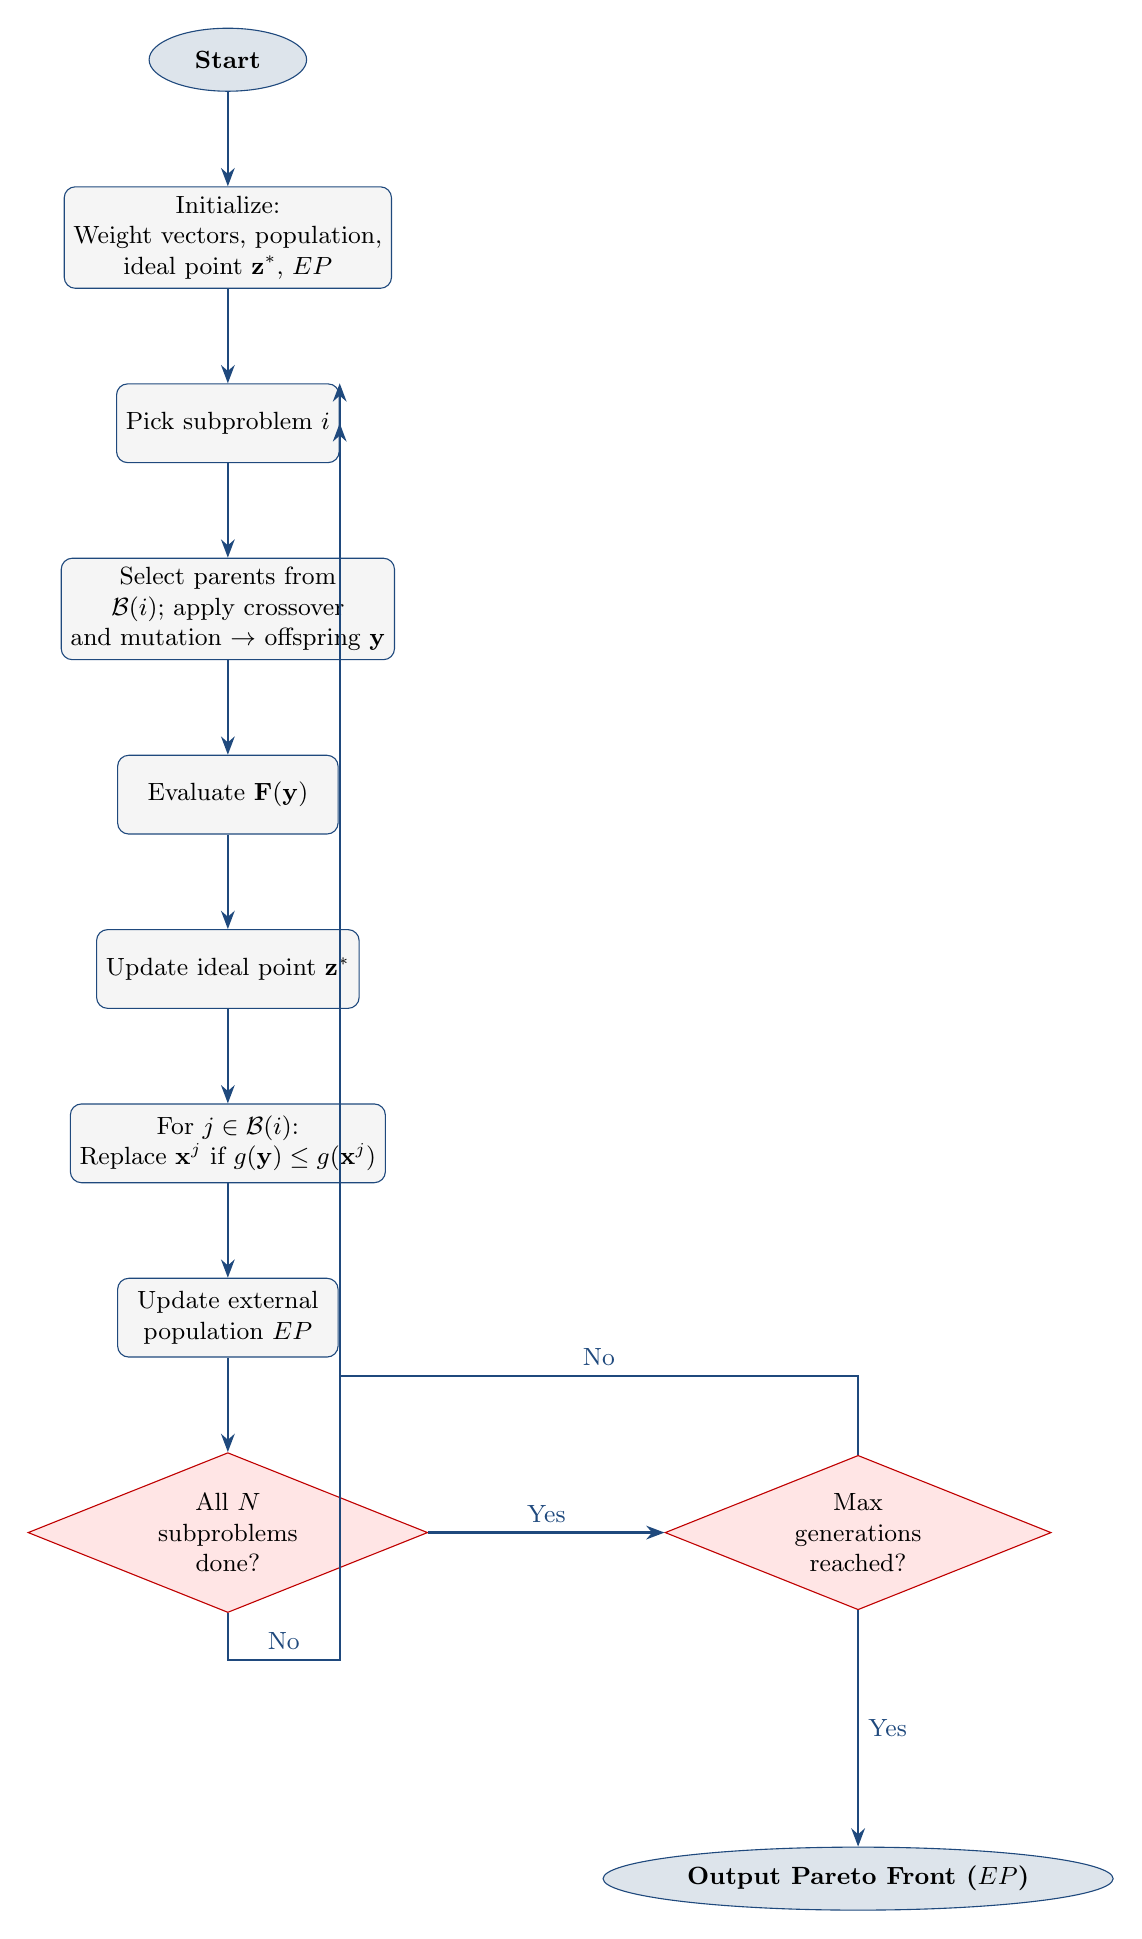
\begin{tikzpicture}[node distance=1.2cm, every node/.style={font=\small}]
    \node[startend] (start) {Start};
    \node[block, below=of start] (init) {Initialize:\\Weight vectors, population,\\ideal point $\mathbf{z}^*$, $EP$};
    \node[block, below=of init] (pick) {Pick subproblem $i$};
    \node[block, below=of pick] (repro) {Select parents from\\$\mathcal{B}(i)$; apply crossover\\and mutation $\rightarrow$ offspring $\mathbf{y}$};
    \node[block, below=of repro] (eval) {Evaluate $\mathbf{F}(\mathbf{y})$};
    \node[block, below=of eval] (update_z) {Update ideal point $\mathbf{z}^*$};
    \node[block, below=of update_z] (update_nb) {For $j \in \mathcal{B}(i)$:\\Replace $\mathbf{x}^j$ if $g(\mathbf{y}) \leq g(\mathbf{x}^j)$};
    \node[block, below=of update_nb] (update_ep) {Update external\\population $EP$};
    \node[decision, below=of update_ep] (all_sub) {All $N$\\subproblems\\done?};
    \node[decision, right=3cm of all_sub] (max_gen) {Max\\generations\\reached?};
    \node[startend, below=3cm of max_gen] (out) {Output Pareto Front ($EP$)};

    \draw[arrow] (start) -- (init);
    \draw[arrow] (init) -- (pick);
    \draw[arrow] (pick) -- (repro);
    \draw[arrow] (repro) -- (eval);
    \draw[arrow] (eval) -- (update_z);
    \draw[arrow] (update_z) -- (update_nb);
    \draw[arrow] (update_nb) -- (update_ep);
    \draw[arrow] (update_ep) -- (all_sub);
    \draw[arrow] (all_sub.east) -- node[above]{\small Yes} (max_gen.west);
    \draw[arrow] (all_sub.south) -- ++(0,-0.6) -| node[above, near start]{\small No} (pick.east);
    \draw[arrow] (max_gen.south) -- node[right]{\small Yes} (out);
    \draw[arrow] (max_gen.north) -- ++(0,1) -| node[above, near start]{\small No} (pick.north east);
\end{tikzpicture}
\caption{Complete flowchart of the MOEA/D algorithm.}
\label{fig:moead_flowchart}
\end{figure}

\subsection{Step-by-Step Walkthrough: The Five Friends}

To make the algorithm concrete, consider five friends looking to buy the best car, each with a different price--quality preference:

\begin{table}[H]
\centering
\caption{Five friends as five MOEA/D subproblems}
\label{tab:five_friends}
\renewcommand{\arraystretch}{1.3}
\begin{tabular}{ccccc}
\toprule
\textbf{Friend (Subproblem)} & $\boldsymbol{\lambda}$ (Quality, Price) & \textbf{Focus} & \textbf{Neighbors} \\
\midrule
F1 & (0.9, 0.1) & Quality first & F2 \\
F2 & (0.7, 0.3) & Good quality  & F1, F3 \\
F3 & (0.5, 0.5) & Balanced      & F2, F4 \\
F4 & (0.3, 0.7) & Cheaper car   & F3, F5 \\
F5 & (0.1, 0.9) & Cheapest      & F4 \\
\bottomrule
\end{tabular}
\end{table}

\textbf{Step 1 --- Initialization:} Each friend randomly picks one car.

\textbf{Step 2 --- Reproduction:} Friend F3 (balanced) looks at F2 and F4. It takes parts from their current cars via crossover to create a new Car D, then applies mutation (a small tweak). Car D: Quality = 80, Price = \$20k.

\textbf{Step 3 --- Neighborhood Update:} F3 shares Car D with neighbors F2 and F4. Each evaluates Car D using their own weight vector:
\begin{align}
    g^{\text{WS}}(\text{Car D} \mid \boldsymbol{\lambda}^{F2}) &= 0.7 \times 80 + 0.3 \times (-20) = 50 \quad \text{(using negated price as quality)}
\end{align}

If Car D's score is better than the neighbor's current solution, the neighbor adopts Car D. One good discovery can propagate to multiple subproblems.

\textbf{Step 4 --- Repeat:} Each friend takes a turn every generation. After many generations, each friend converges to the best possible car for their preference --- yielding one point on the Pareto front per subproblem.

\subsection{Scoring Under Tchebycheff: Numerical Example}

Suppose $m = 2$, $\mathbf{z}^* = (0, 0)$ (ideal), and we compare Car C and Car D for subproblem $i$ with $\boldsymbol{\lambda}^i = (0.5, 0.5)$:

\begin{align}
    \mathbf{F}(\text{Car C}) &= (f_1, f_2) = (4, -150), \quad
    g^{\text{TCH}} = \max(0.5 \cdot |4 - 0|,\; 0.5 \cdot |-150 - 0|) = 75, \\[4pt]
    \mathbf{F}(\text{Car D}) &= (f_1, f_2) = (20, -80), \quad
    g^{\text{TCH}} = \max(0.5 \cdot |20|,\; 0.5 \cdot 80) = 40.
\end{align}

Car D achieves a lower Tchebycheff score, so it replaces Car C for this balanced subproblem.

% =============================================================
\section{Key Design Parameters}
\label{sec:design}
% =============================================================

\subsection{Number of Subproblems $N$}

$N$ controls the density of coverage of the Pareto front. Too few subproblems leave large gaps in the front; too many increase computational cost. A common choice is $N \in [100, 300]$ for two-objective problems.

\begin{figure}[H]
\centering
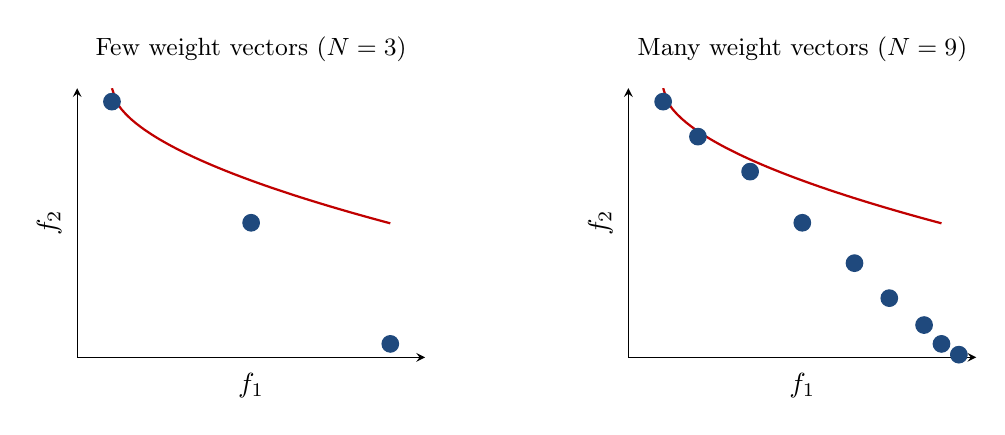
\begin{tikzpicture}
    \begin{scope}[xshift=0cm]
        \begin{axis}[
            width=6cm, height=5cm,
            title={\small Few weight vectors ($N=3$)},
            xlabel={$f_1$}, ylabel={$f_2$},
            xmin=0, xmax=10, ymin=0, ymax=10,
            xtick=\empty, ytick=\empty,
            axis lines=left
        ]
        \addplot[thick, color=paretored, domain=1:9, samples=60]
            {10 - (x-1)^(0.55)*1.6};
        \addplot[only marks, mark=*, color=primaryblue, mark size=3]
            coordinates{(1,9.5)(5,5)(9,0.5)};
        \end{axis}
    \end{scope}
    \begin{scope}[xshift=7cm]
        \begin{axis}[
            width=6cm, height=5cm,
            title={\small Many weight vectors ($N=9$)},
            xlabel={$f_1$}, ylabel={$f_2$},
            xmin=0, xmax=10, ymin=0, ymax=10,
            xtick=\empty, ytick=\empty,
            axis lines=left
        ]
        \addplot[thick, color=paretored, domain=1:9, samples=60]
            {10 - (x-1)^(0.55)*1.6};
        \addplot[only marks, mark=*, color=primaryblue, mark size=3]
            coordinates{(1,9.5)(2,8.2)(3.5,6.9)(5,5)(6.5,3.5)(7.5,2.2)(8.5,1.2)(9,0.5)(9.5,0.1)};
        \end{axis}
    \end{scope}
\end{tikzpicture}
\caption{Effect of the number of weight vectors on Pareto front coverage.}
\label{fig:coverage}
\end{figure}

\subsection{Neighborhood Size $T$}

The neighborhood size $T$ determines how many subproblems cooperate. A small $T$ gives each subproblem more focused, targeted optimization but may reduce diversity. A large $T$ increases information sharing but may cause premature convergence. Typical values: $T = \lfloor 0.1 N \rfloor$ to $\lfloor 0.2 N \rfloor$.

\subsection{Ideal Reference Point $\mathbf{z}^*$}

For TCH scalarization, $z_k^* = \min_i f_k(\mathbf{x}^i)$ is maintained dynamically and updated whenever a solution achieves a new best on any objective. An inaccurate $\mathbf{z}^*$ (overestimated) does not break correctness but may slow convergence.

\subsection{Weight Vector Generation}

For two objectives, weight vectors are uniformly spaced:
\begin{equation}
    \boldsymbol{\lambda}^i = \Bigl(\frac{i-1}{N-1},\; 1 - \frac{i-1}{N-1}\Bigr), \quad i = 1, \ldots, N.
\end{equation}

For $m \geq 3$ objectives, systematic simplex-lattice designs (e.g., Das--Dennis approach) or random uniform sampling on the unit simplex are used.

\begin{table}[H]
\centering
\caption{Summary of key MOEA/D hyperparameters}
\label{tab:hyperparams}
\renewcommand{\arraystretch}{1.4}
\begin{tabular}{cccp{5cm}}
\toprule
\textbf{Parameter} & \textbf{Symbol} & \textbf{Typical Value} & \textbf{Effect} \\
\midrule
Number of subproblems & $N$ & 100--300 & Controls front coverage density \\
Neighborhood size & $T$ & $0.1N$--$0.2N$ & Balances convergence vs.\ diversity \\
Max generations & $G$ & 500--1000 & Determines runtime budget \\
Distribution index (SBX) & $\eta_c$ & 20 & Controls crossover spread \\
Mutation index & $\eta_m$ & 20 & Controls mutation step size \\
PBI penalty & $\theta$ & 5 & Trades convergence for diversity \\
\bottomrule
\end{tabular}
\end{table}

% =============================================================
\section{Why Decomposition Is Powerful: Three Key Advantages}
\label{sec:advantages}
% =============================================================

\subsection{Local Focus}

Without decomposition, every solution competes globally against all others in the population. The fitness landscape becomes complex and directionless. With decomposition, each subproblem has a clear scalar objective $g^i$, narrowing the search to a single direction. This local focus accelerates convergence per subproblem.

\subsection{Natural Diversity}

Because subproblems span many different search directions (weight vectors), the solutions they find naturally spread across the Pareto front. No special diversity preservation mechanism (e.g., crowding distance as in NSGA-II) is needed --- diversity is an inherent consequence of the decomposition strategy.

\subsection{No Global Ranking Required}

Pareto-dominance-based methods (e.g., NSGA-II) require sorting all solutions by dominance rank, which costs $O(mN^2)$ per generation for $m$ objectives and $N$ solutions. MOEA/D replaces this with simple scalar comparisons ($g^i(\mathbf{y}) \leq g^i(\mathbf{x}^j)$?), reducing per-generation complexity dramatically.

\begin{table}[H]
\centering
\caption{Three advantages of decomposition in MOEA/D}
\label{tab:advantages}
\renewcommand{\arraystretch}{1.4}
\begin{tabular}{p{3cm} p{5.5cm} p{5cm}}
\toprule
\textbf{Advantage} & \textbf{Without Decomposition} & \textbf{With Decomposition} \\
\midrule
Focus & Global, unfocused search & Each subproblem has one clear direction \\
Diversity & Requires explicit diversity preservation & Diversity is automatic \\
Complexity & $O(mN^2)$ per generation (dominance sort) & $O(NT)$ per generation (scalar comparisons) \\
\bottomrule
\end{tabular}
\end{table}

% =============================================================
\section{Comparison with Related Algorithms}
\label{sec:comparison}
% =============================================================

\subsection{MOEA/D vs.\ NSGA-II}

NSGA-II (Non-dominated Sorting Genetic Algorithm II) is one of the most widely used MOEAs. Table~\ref{tab:nsga_moead} compares the two algorithms.

\begin{table}[H]
\centering
\caption{MOEA/D vs.\ NSGA-II: a detailed comparison}
\label{tab:nsga_moead}
\renewcommand{\arraystretch}{1.4}
\begin{tabular}{>{\bfseries}p{3.5cm} p{5cm} p{5cm}}
\toprule
\textbf{Aspect} & \textbf{NSGA-II} & \textbf{MOEA/D} \\
\midrule
Core mechanism & Dominance-based sorting + crowding distance & Decomposition + neighborhood cooperation \\
Selection & Tournament on rank and crowding & Neighbor-based selection \\
Diversity maintenance & Crowding distance (explicit) & Weight vector spread (implicit) \\
Scalarization & None & Weighted Sum / Tchebycheff / PBI \\
Complexity per generation & $O(mN^2)$ & $O(NT)$ \\
Non-convex fronts & Handles well & Handles well (TCH/PBI) \\
Many objectives ($m>3$) & Degrades significantly & More scalable \\
External population & No (inline) & Optional ($EP$) \\
Year proposed & 2002 (Deb et al.) & 2007 (Zhang \& Li) \\
\bottomrule
\end{tabular}
\end{table}

\subsection{MOEA/D vs.\ Weighted Sum Method}

The naive weighted sum method fixes weights and runs a single-objective optimizer repeatedly. MOEA/D uses all weight vectors simultaneously in a cooperative population, allowing solutions from one weight direction to benefit neighboring directions. This collaborative aspect is fundamentally absent in independent multi-run weighted sum.

\subsection{MOEA/D vs.\ MOEA/D Variants}

Several extensions of MOEA/D have been developed:

\begin{table}[H]
\centering
\caption{MOEA/D variants and their contributions}
\label{tab:moead_variants}
\renewcommand{\arraystretch}{1.3}
\begin{tabular}{p{3.5cm} p{9cm}}
\toprule
\textbf{Variant} & \textbf{Key Contribution} \\
\midrule
MOEA/D-DE & Replaces SBX crossover with Differential Evolution operators for better exploration \\
MOEA/D-DRA & Dynamic Resource Allocation: adaptively assigns computational budget to harder subproblems \\
MOEA/D-M2M & Divides the population into multiple sub-populations for irregular Pareto fronts \\
MOEA/D-AWA & Adaptive weight adjustment for non-uniform Pareto fronts \\
MOEA/D-STM & Stable matching model for assignment of offspring to subproblems \\
\bottomrule
\end{tabular}
\end{table}

% =============================================================
\section{Performance Metrics}
\label{sec:metrics}
% =============================================================

Evaluating how well a multi-objective algorithm approximates the true Pareto front requires specific metrics.

\subsection{Generational Distance (GD)}

GD measures the average distance from the obtained solution set $P$ to the true Pareto front $PF^*$:
\begin{equation}
    \text{GD}(P, PF^*) = \frac{1}{|P|} \sqrt{ \sum_{\mathbf{v} \in P} d(\mathbf{v}, PF^*)^2 },
\end{equation}
where $d(\mathbf{v}, PF^*)$ is the Euclidean distance from point $\mathbf{v}$ to the nearest point in $PF^*$. Lower GD $\Rightarrow$ better \textbf{convergence}.

\subsection{Inverted Generational Distance (IGD)}

IGD measures the average distance from the true front to the obtained set:
\begin{equation}
    \text{IGD}(P, PF^*) = \frac{1}{|PF^*|} \sqrt{ \sum_{\mathbf{u} \in PF^*} d(\mathbf{u}, P)^2 }.
\end{equation}
IGD captures both convergence and diversity simultaneously. It is widely used as a primary benchmark metric.

\subsection{Hypervolume (HV)}

The hypervolume indicator measures the $m$-dimensional volume dominated by the obtained solution set $P$ and bounded by a reference point $\mathbf{r}$:
\begin{equation}
    \text{HV}(P, \mathbf{r}) = \lambda_m\!\left( \bigcup_{\mathbf{p} \in P} [\mathbf{p}, \mathbf{r}] \right),
\end{equation}
where $\lambda_m$ is the Lebesgue measure. Higher HV $\Rightarrow$ better (more area dominated). HV is the only unary metric that captures both convergence and diversity.

\begin{table}[H]
\centering
\caption{Summary of Pareto front quality metrics}
\label{tab:metrics}
\renewcommand{\arraystretch}{1.3}
\begin{tabular}{p{3cm} p{4cm} p{3cm} p{3cm}}
\toprule
\textbf{Metric} & \textbf{Measures} & \textbf{Best value} & \textbf{Reference needed?} \\
\midrule
GD  & Convergence & 0 (lower better) & True PF \\
IGD & Convergence + Diversity & 0 (lower better) & True PF \\
HV  & Convergence + Diversity & max (higher better) & Reference point \\
Spread $\Delta$ & Diversity only & 0 (lower better) & True PF \\
\bottomrule
\end{tabular}
\end{table}

% =============================================================
\section{Image Placeholders}
\label{sec:images}
% =============================================================

The following figures are referenced throughout the report. Please insert the corresponding images as indicated:

\begin{figure}[H]
\centering
\fbox{\parbox{0.8\textwidth}{\centering\vspace{2cm}
\textbf{[PLACEHOLDER: Pareto front evolution over generations]}\\[0.3em]
\small Insert a figure showing how the population evolves from a random scatter (Generation 0) through intermediate generations (Gen 1, 2) to a converged Pareto front. The figure should be a 4-panel image: Gen 0 (scattered), Gen 1 (shifting), Gen 2 (converging), Converged (Pareto front).\\[0.3em]
Suggested source: Generate using MATLAB/Python MOEA/D implementation on ZDT1 test function.
\vspace{2cm}}}
\caption{Evolution of the population across generations, showing convergence toward the Pareto front.}
\label{fig:gen_evolution}
\end{figure}

\begin{figure}[H]
\centering
\fbox{\parbox{0.8\textwidth}{\centering\vspace{2cm}
\textbf{[PLACEHOLDER: MOEA/D neighborhood cooperation diagram]}\\[0.3em]
\small A diagram showing $N=5$ subproblems arranged in a line or circle, with arrows between neighbors indicating information sharing. Each subproblem labeled with its weight vector $\boldsymbol{\lambda}^i$. Arrows highlighted in red where a good offspring has been shared.\\[0.3em]
Suggested tool: Draw using TikZ or any diagram editor.
\vspace{2cm}}}
\caption{Neighborhood cooperation in MOEA/D: each subproblem shares discovered solutions with its $T$ nearest neighbors.}
\label{fig:neighborhood}
\end{figure}

\begin{figure}[H]
\centering
\fbox{\parbox{0.8\textwidth}{\centering\vspace{2cm}
\textbf{[PLACEHOLDER: MOEA/D vs. NSGA-II Pareto front comparison on ZDT1]}\\[0.3em]
\small A side-by-side plot: left shows NSGA-II result (blue dots) vs.\ true PF (red curve); right shows MOEA/D result (blue dots) vs.\ true PF. Axes: $f_1$ (x-axis), $f_2$ (y-axis). Both run for the same number of function evaluations (e.g., 30,000).\\[0.3em]
Suggested source: Run both algorithms on ZDT1 benchmark using PlatEMO or jMetal.
\vspace{2cm}}}
\caption{Comparative Pareto front approximation: NSGA-II (left) vs.\ MOEA/D (right) on the ZDT1 benchmark.}
\label{fig:comparison_plot}
\end{figure}

\begin{figure}[H]
\centering
\fbox{\parbox{0.8\textwidth}{\centering\vspace{2cm}
\textbf{[PLACEHOLDER: Three-objective Pareto front surface]}\\[0.3em]
\small A 3D scatter plot of the Pareto front for a three-objective problem (e.g., DTLZ1). Axes: $f_1$, $f_2$, $f_3$. Points colored by a gradient from blue (low $f_1$) to red (high $f_1$) to show the trade-off surface. Generated by MOEA/D with $N = 300$ subproblems.\\[0.3em]
Suggested source: PlatEMO DTLZ1 with MOEA/D-TCH, 3 objectives.
\vspace{2cm}}}
\caption{Three-dimensional Pareto front for a DTLZ1-type problem, approximated by MOEA/D.}
\label{fig:3d_pareto}
\end{figure}

% =============================================================
\section{Applications of MOEA/D}
\label{sec:applications}
% =============================================================

MOEA/D has been applied to a wide range of real-world engineering and scientific problems. Table~\ref{tab:applications} summarizes notable application domains.

\begin{table}[H]
\centering
\caption{Real-world applications of MOEA/D}
\label{tab:applications}
\renewcommand{\arraystretch}{1.3}
\begin{tabular}{p{3.5cm} p{4cm} p{5.5cm}}
\toprule
\textbf{Domain} & \textbf{Objectives} & \textbf{Notes} \\
\midrule
Vehicle design & Minimize weight, fuel use; maximize safety & Conflicting structural and performance goals \\
Wireless networks & Maximize throughput; minimize energy use & Resource allocation in 5G/IoT \\
Chemical engineering & Maximize yield; minimize cost and waste & Multi-reactor process optimization \\
Portfolio optimization & Maximize return; minimize risk (variance) & Markowitz mean-variance model extended \\
Neural architecture search & Maximize accuracy; minimize model size & Hardware-constrained AI deployment \\
Water distribution & Minimize cost; minimize water loss & Infrastructure resilience trade-offs \\
Medical treatment planning & Minimize tumor dose error; minimize healthy tissue exposure & Radiotherapy optimization \\
Power systems & Minimize generation cost; minimize emissions & Economic--environmental dispatch \\
\bottomrule
\end{tabular}
\end{table}

% =============================================================
\section{Limitations and Open Challenges}
\label{sec:limitations}
% =============================================================

Despite its effectiveness, MOEA/D has several known limitations:

\begin{enumerate}[leftmargin=1.5cm]
    \item \textbf{Many-objective scalability:} For $m > 4$ objectives, uniformly distributing weight vectors becomes difficult. The number of weight vectors needed to cover the simplex grows combinatorially with $m$.

    \item \textbf{Irregular Pareto fronts:} MOEA/D assumes that uniformly distributed weight vectors lead to uniformly distributed Pareto solutions. On problems with disconnected or degenerate Pareto fronts, some weight directions may find no good solutions while others find many.

    \item \textbf{Sensitivity to scalarization choice:} WS fails on non-convex fronts. TCH can produce ``corner solutions'' (extreme trade-offs) that dominate intermediate subproblems, leading to uneven distribution.

    \item \textbf{Hyperparameter tuning:} Performance depends on $N$, $T$, $\theta$, and the crossover/mutation operators. Automatic hyperparameter adaptation is an active research area.

    \item \textbf{Constraint handling:} Standard MOEA/D does not natively handle hard constraints; constraint-handling techniques (e.g., penalty functions, $\epsilon$-constraint method) must be incorporated separately.
\end{enumerate}

% =============================================================
\section{Worked Example: MOEA/D on a 2D MOP}
\label{sec:example}
% =============================================================

\subsection{Problem Setup}

Consider the ZDT1 benchmark function (a standard 2-objective test problem):
\begin{align}
    \min\; f_1(\mathbf{x}) &= x_1, \\
    \min\; f_2(\mathbf{x}) &= g(\mathbf{x}) \cdot \left[1 - \sqrt{\frac{x_1}{g(\mathbf{x})}}\right], \\
    g(\mathbf{x}) &= 1 + \frac{9}{n-1}\sum_{i=2}^{n} x_i, \quad
    \mathbf{x} \in [0,1]^n, \; n = 30.
\end{align}

The true Pareto front is $f_2 = 1 - \sqrt{f_1}$ for $f_1 \in [0,1]$ --- a convex curve.

\subsection{MOEA/D Configuration}

\begin{itemize}[leftmargin=1.5cm]
    \item $N = 100$ uniformly spaced weight vectors: $\boldsymbol{\lambda}^i = (i/N, 1 - i/N)$, $i = 0, \ldots, N$.
    \item Neighborhood size $T = 10$.
    \item Scalarization: Tchebycheff.
    \item Crossover: SBX ($\eta_c = 20$), Mutation: Polynomial ($\eta_m = 20$, $p_m = 1/n$).
    \item Max generations: 500.
\end{itemize}

\subsection{Expected Behavior}

At generation 0, solutions are randomly distributed in $[0,1]^2$ in objective space, with poor objective values. By generation 50, the neighborhood cooperation pushes solutions toward the true front. By generation 200, MOEA/D achieves a well-spread, dense approximation of $f_2 = 1 - \sqrt{f_1}$ with IGD $< 0.01$.

% =============================================================
\section{Mathematical Summary}
\label{sec:math_summary}
% =============================================================

Table~\ref{tab:math_summary} consolidates the key mathematical definitions and equations presented in this report.

\begin{table}[H]
\centering
\caption{Key equations in MOEA/D}
\label{tab:math_summary}
\renewcommand{\arraystretch}{1.6}
\begin{tabular}{p{4cm} p{10cm}}
\toprule
\textbf{Concept} & \textbf{Equation} \\
\midrule
MOP formulation & $\min_{\mathbf{x} \in \Omega} \mathbf{F}(\mathbf{x}) = (f_1(\mathbf{x}), \ldots, f_m(\mathbf{x}))$ \\
Dominance & $\mathbf{x}^{(1)} \prec \mathbf{x}^{(2)} \Leftrightarrow f_k(\mathbf{x}^{(1)}) \leq f_k(\mathbf{x}^{(2)})\;\forall k$ and $\exists j: f_j(\mathbf{x}^{(1)}) < f_j(\mathbf{x}^{(2)})$ \\
Ideal point & $z_k^* = \min_{\mathbf{x}} f_k(\mathbf{x}), \quad k = 1, \ldots, m$ \\
Weight constraint & $\sum_{k=1}^m \lambda_k = 1, \quad \lambda_k \geq 0$ \\
WS scalarization & $g^{\text{WS}} = \sum_{k=1}^m \lambda_k f_k(\mathbf{x})$ \\
TCH scalarization & $g^{\text{TCH}} = \max_{k} \lambda_k |f_k(\mathbf{x}) - z_k^*|$ \\
PBI scalarization & $g^{\text{PBI}} = d_1 + \theta d_2$ \\
Neighborhood & $\mathcal{B}(i) = \{j : \boldsymbol{\lambda}^j \text{ among } T \text{ nearest to } \boldsymbol{\lambda}^i\}$ \\
GD metric & $\text{GD} = \frac{1}{|P|}\sqrt{\sum_{\mathbf{v}\in P} d(\mathbf{v}, PF^*)^2}$ \\
IGD metric & $\text{IGD} = \frac{1}{|PF^*|}\sqrt{\sum_{\mathbf{u}\in PF^*} d(\mathbf{u}, P)^2}$ \\
HV metric & $\text{HV}(P,\mathbf{r}) = \lambda_m\!\left(\bigcup_{\mathbf{p}\in P}[\mathbf{p},\mathbf{r}]\right)$ \\
\bottomrule
\end{tabular}
\end{table}

% =============================================================
\section{Conclusion}
\label{sec:conclusion}
% =============================================================

MOEA/D represents a significant milestone in the field of multi-objective evolutionary computation. By decomposing a single complex multi-objective problem into $N$ simpler scalar subproblems --- each with its own preference direction encoded as a weight vector --- and enabling cooperative information sharing among neighboring subproblems, MOEA/D achieves an efficient and well-distributed approximation of the Pareto front in a single run.

The key contributions of MOEA/D can be summarized as follows:

\begin{enumerate}[leftmargin=1.5cm]
    \item \textbf{Decomposition:} The paradigm shift from global dominance-based ranking to local scalar optimization dramatically simplifies each individual search task and reduces computational complexity from $O(mN^2)$ to $O(NT)$ per generation.

    \item \textbf{Scalarization flexibility:} Support for multiple scalarization approaches (WS, TCH, PBI) makes MOEA/D adaptable to a wide variety of Pareto front shapes, including both convex and non-convex fronts.

    \item \textbf{Neighborhood cooperation:} The exploitation of similarity among neighboring subproblems enables efficient propagation of good solutions, accelerating convergence without sacrificing diversity.

    \item \textbf{Built-in diversity:} Unlike algorithms that require explicit diversity-preservation mechanisms, diversity in MOEA/D arises naturally from the uniform distribution of weight vectors across the objective space.

    \item \textbf{Practical impact:} MOEA/D has been successfully applied to vehicle design, neural architecture search, water system management, portfolio optimization, and many other domains where conflicting objectives are the norm rather than the exception.
\end{enumerate}

As Henry Ford once said: \textit{``Nothing is particularly hard if you divide it into small jobs.''} MOEA/D embodies this philosophy, turning the intractable task of global multi-objective search into a collection of manageable, cooperative scalar optimizations. It remains one of the most influential frameworks in evolutionary multi-objective optimization and continues to inspire extensions and applications across science and engineering.

% =============================================================
% References
% =============================================================
\newpage
\begin{thebibliography}{99}

\bibitem{zhang2007}
Q. Zhang and H. Li,
``MOEA/D: A Multiobjective Evolutionary Algorithm Based on Decomposition,''
\textit{IEEE Transactions on Evolutionary Computation}, vol. 11, no. 6, pp. 712--731, Dec. 2007.

\bibitem{deb2002}
K. Deb, A. Pratap, S. Agarwal, and T. Meyarivan,
``A fast and elitist multiobjective genetic algorithm: NSGA-II,''
\textit{IEEE Transactions on Evolutionary Computation}, vol. 6, no. 2, pp. 182--197, Apr. 2002.

\bibitem{miettinen1999}
K. Miettinen,
\textit{Nonlinear Multiobjective Optimization}.
Springer, 1999.

\bibitem{zitzler2000}
E. Zitzler, K. Deb, and L. Thiele,
``Comparison of Multiobjective Evolutionary Algorithms: Empirical Results,''
\textit{Evolutionary Computation}, vol. 8, no. 2, pp. 173--195, 2000.

\bibitem{li2009}
H. Li and Q. Zhang,
``Multiobjective Optimization Problems with Complicated Pareto Sets, MOEA/D and NSGA-II,''
\textit{IEEE Transactions on Evolutionary Computation}, vol. 13, no. 2, pp. 284--302, Apr. 2009.

\bibitem{ishibuchi2017}
H. Ishibuchi, R. Imada, Y. Setoguchi, and Y. Nojima,
``Performance of Decomposition-Based Many-Objective Algorithms Strongly Depends on Pareto Front Shapes,''
\textit{IEEE Transactions on Evolutionary Computation}, vol. 21, no. 2, pp. 169--190, 2017.

\bibitem{zhang2009}
Q. Zhang, W. Liu, and H. Li,
``The Performance of a New Version of MOEA/D on CEC09 Unconstrained MOP Test Instances,''
\textit{IEEE Congress on Evolutionary Computation (CEC)}, 2009, pp. 203--208.

\bibitem{cai2015}
X. Cai, Z. Mei, Z. Fan, and Q. Zhang,
``A Constrained Decomposition Approach with Grids for Evolutionary Multiobjective Optimization,''
\textit{IEEE Transactions on Evolutionary Computation}, vol. 22, no. 4, pp. 564--577, 2018.

\end{thebibliography}

\end{document}